\documentclass{beamer}
\usetheme{Madrid}
\usepackage{graphicx}
\usepackage{amsmath}
\usepackage{booktabs}
\usepackage{array}

\title{Statically Indeterminate Axially Loaded Members}
\subtitle{Week 4}
\author{Viggo K. Hansen}
\institute{ISE}

\begin{document}

\begin{frame}
    \titlepage
\end{frame}

\begin{frame}
    \frametitle{Chapter Objectives}
    \begin{itemize}
        \item Determine deformation of axially loaded members.
        \item Analyze support reactions in statically indeterminate systems.
        \item Analyze the effects of thermal stress.
        \item Discuss inelastic deformation and residual stress.
    \end{itemize}
\end{frame}

\begin{frame}
    \frametitle{Review of Axially Loaded Members}
    \begin{itemize}
        \item \textbf{Normal stress}: $\sigma = \frac{P}{A}$
        \item Axial force ($P$) and its sign convention:
            \begin{itemize}
                \item Tension: Positive ($P > 0$)
                \item Compression: Negative ($P < 0$)
            \end{itemize}
        \item Cross-sectional area ($A$)
        \item Elastic deformation: $\delta = \frac{PL}{AE}$ (for elastic deformation under uniaxial load, this is a simplified form assuming linear elasticity)
    \end{itemize}
\end{frame}

\begin{frame}
    \frametitle{Definition of Statically Indeterminate Members}
    \begin{itemize}
        \item \textbf{Static Indeterminacy}: 
        \begin{itemize}
            \item Equilibrium equations are insufficient to solve for all unknowns.
            \item More unknown reactions than available equilibrium equations.
            \item Additional equations based on compatibility or material behavior are required for solution. "Compatibility" here refers to the requirement that displacements must be consistent with the boundary conditions of the system.
        \end{itemize}
    \end{itemize}
\end{frame}

\begin{frame}
    \frametitle{Examples of Statically Indeterminate Systems}
    \begin{itemize}
        \item A bar fixed at both ends.
        \item A bar with multiple supports.
        \item A composite structure with axial loading (note that these often involve different materials with distinct moduli of elasticity, requiring careful analysis using both equilibrium and compatibility conditions).
    \end{itemize}
    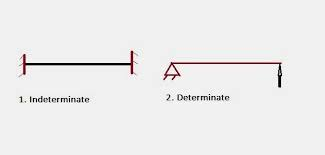
\includegraphics[width=0.5\textwidth]{download.jpg}
\end{frame}

\begin{frame}
    \frametitle{General Procedure for Analysis}
    \begin{enumerate}
        \item \textbf{Equilibrium}: 
            \begin{itemize}
                \item Draw Free Body Diagrams (FBDs).
                \item Write equilibrium equations.
            \end{itemize}
        \item \textbf{Compatibility}: 
            \begin{itemize}
                \item Analyze how the structure deforms.
            \end{itemize}
        \item \textbf{Force-Displacement Relations}: 
            \begin{itemize}
                \item Relate forces and deformations using material properties. These relations can involve concepts like Hooke's Law for linear elasticity or more complex relationships in case of non-linear behavior.
            \end{itemize}
        \item Solve equations simultaneously.
    \end{enumerate}
\end{frame}

\begin{frame}
    \frametitle{Compatibility Equations}
    \begin{itemize}
        \item Displacements or deformations must be consistent with constraints.
        \item Relate the deformation in each segment of the structure:
            \[
            \delta_{A/B} = \delta_A - \delta_B
            \]
            This equation ensures that the displacements at points A and B match in a way that maintains the structure's integrity.
    \end{itemize}
\end{frame}

\begin{frame}
    \frametitle{Example Problem 1 - Bar Fixed at Both Ends}
    \begin{itemize}
        \item A bar fixed at both ends with an axial load $P$.
        \item Free Body Diagram:
        \begin{figure}
            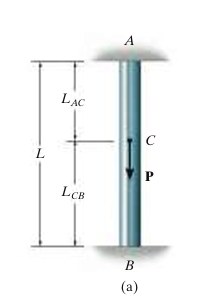
\includegraphics[width=0.2\textwidth]{Beam.png}
        \end{figure}
        \item Equilibrium: $\sum F_x = 0 \rightarrow F_A + F_B - P = 0$ (where $F_A$ and $F_B$ are the internal forces at the ends of the bar)
        \item Compatibility: $\delta_{A/B} = 0$
    \end{itemize}
\end{frame}

\begin{frame}
    \frametitle{Example Problem 1 - Solution}
    \begin{itemize}
        \item Using $\delta = \frac{FL}{AE}$:
            \[
            \delta_{A/B} = \frac{F_A L_{AC}}{AE} - \frac{F_B L_{CB}}{AE} = 0
            \]
            Here, $\delta_{A/B}$ is the total displacement at the point of interest due to the internal forces.
        \item Solving for $F_A$ and $F_B$ (ensure $L_{AC}$ and $L_{CB}$ are well-defined in the problem statement):
            \[
            F_A = P \left(\frac{L_{CB}}{L}\right), \quad F_B = P \left(\frac{L_{AC}}{L}\right)
            \]
    \end{itemize}
\end{frame}

\begin{frame}
    \frametitle{Thermal Stress}
    \begin{itemize}
        \item Temperature changes cause expansion or contraction.
        \item If movement is constrained, thermal stress develops.
        \item Thermal strain: $\epsilon_T = \alpha \Delta T$ where $\alpha$ is the coefficient of thermal expansion and $\Delta T$ is the temperature change.
        \item Thermal stress is only relevant when the material is restrained from free expansion or contraction.
    \end{itemize}
\end{frame}

\begin{frame}
    \frametitle{Conclusion}
    \begin{itemize}
        \item Statically indeterminate members require additional compatibility equations.
        \item Thermal stress analysis is essential in many applications.
        \item Inelastic deformation leads to residual stress, which can arise from plastic deformations that are often irreversible.
        \item Superposition is a valuable tool for linear elastic problems.
    \end{itemize}
\end{frame}

\end{document}